% !TeX encoding = UTF-8
% !TeX spellcheck = es_ES
% !TeX root = main.tex

%%%%%%%%%%%%%%%%%%%%%%%%%%%%%%%%%%%%%%%%%
% The Legrand Orange Book
% LaTeX Template
% Version 2.4 (26/09/2018)
%
% This template was downloaded from:
% http://www.LaTeXTemplates.com
%
% Original author:
% Mathias Legrand (legrand.mathias@gmail.com) with modifications by:
% Vel (vel@latextemplates.com)
%
% License:
% CC BY-NC-SA 3.0 (http://creativecommons.org/licenses/by-nc-sa/3.0/)
%
% Compiling this template:
% This template uses biber for its bibliography and makeindex for its index.
% When you first open the template, compile it from the command line with the 
% commands below to make sure your LaTeX distribution is configured correctly:
%
% 1) pdflatex main
% 2) makeindex main.idx -s StyleInd.ist
% 3) biber main
% 4) pdflatex main x 2
%
% After this, when you wish to update the bibliography/index use the appropriate
% command above and make sure to compile with pdflatex several times 
% afterwards to propagate your changes to the document.
%
% This template also uses a number of packages which may need to be
% updated to the newest versions for the template to compile. It is strongly
% recommended you update your LaTeX distribution if you have any
% compilation errors.
%
% Important note:
% Chapter heading images should have a 2:1 width:height ratio,
% e.g. 920px width and 460px height.
%
%%%%%%%%%%%%%%%%%%%%%%%%%%%%%%%%%%%%%%%%%

%----------------------------------------------------------------------------------------
%	PACKAGES AND OTHER DOCUMENT CONFIGURATIONS
%----------------------------------------------------------------------------------------

\documentclass[11pt,fleqn]{book} % Default font size and left-justified equations

%%%%%%%%%%%%%%%%%%%%%%%%%%%%%%%%%%%%%%%%%
% The Legrand Orange Book
% Structural Definitions File
% Version 2.1 (26/09/2018)
%
% Original author:
% Mathias Legrand (legrand.mathias@gmail.com) with modifications by:
% Vel (vel@latextemplates.com)
% 
% This file was downloaded from:
% http://www.LaTeXTemplates.com
%
% License:
% CC BY-NC-SA 3.0 (http://creativecommons.org/licenses/by-nc-sa/3.0/)
%
%%%%%%%%%%%%%%%%%%%%%%%%%%%%%%%%%%%%%%%%%

%----------------------------------------------------------------------------------------
%	VARIOUS REQUIRED PACKAGES AND CONFIGURATIONS
%----------------------------------------------------------------------------------------

\usepackage{graphicx} % Required for including pictures
\graphicspath{{Pictures/}} % Specifies the directory where pictures are stored

\usepackage{lipsum} % Inserts dummy text

\usepackage{tikz} % Required for drawing custom shapes

%\usepackage[english]{babel} % English language/hyphenation

\usepackage{enumitem} % Customize lists
\setlist{nolistsep} % Reduce spacing between bullet points and numbered lists

\usepackage{booktabs} % Required for nicer horizontal rules in tables

\usepackage{xcolor} % Required for specifying colors by name
\definecolor{ocre}{RGB}{243,102,25} % Define the orange color used for highlighting throughout the book

%----------------------------------------------------------------------------------------
%	MARGINS
%----------------------------------------------------------------------------------------

\usepackage{geometry} % Required for adjusting page dimensions and margins

\geometry{
	paper=a4paper, % Paper size, change to letterpaper for US letter size
	top=3cm, % Top margin
	bottom=3cm, % Bottom margin
	left=3cm, % Left margin
	right=3cm, % Right margin
	headheight=14pt, % Header height
	footskip=1.4cm, % Space from the bottom margin to the baseline of the footer
	headsep=10pt, % Space from the top margin to the baseline of the header
	%showframe, % Uncomment to show how the type block is set on the page
}

%----------------------------------------------------------------------------------------
%	FONTS
%----------------------------------------------------------------------------------------

\usepackage{avant} % Use the Avantgarde font for headings
%\usepackage{times} % Use the Times font for headings
\usepackage{mathptmx} % Use the Adobe Times Roman as the default text font together with math symbols from the Sym­bol, Chancery and Com­puter Modern fonts

\usepackage{microtype} % Slightly tweak font spacing for aesthetics
\usepackage[utf8]{inputenc} % Required for including letters with accents
\usepackage[T1]{fontenc} % Use 8-bit encoding that has 256 glyphs

%----------------------------------------------------------------------------------------
%	BIBLIOGRAPHY AND INDEX
%----------------------------------------------------------------------------------------

\usepackage[style=numeric,citestyle=numeric,sorting=nyt,sortcites=true,autopunct=true,babel=hyphen,hyperref=true,abbreviate=false,backref=true,backend=biber,refsection=chapter]{biblatex}
\addbibresource{bibliography.bib} % BibTeX bibliography file
\defbibheading{bibempty}{}

\usepackage{calc} % For simpler calculation - used for spacing the index letter headings correctly
\usepackage{makeidx} % Required to make an index
\makeindex % Tells LaTeX to create the files required for indexing

%----------------------------------------------------------------------------------------
%	MAIN TABLE OF CONTENTS
%----------------------------------------------------------------------------------------

\usepackage{titletoc} % Required for manipulating the table of contents

\contentsmargin{0cm} % Removes the default margin

% Part text styling (this is mostly taken care of in the PART HEADINGS section of this file)
\titlecontents{part}
	[0cm] % Left indentation
	{\addvspace{20pt}\bfseries} % Spacing and font options for parts
	{}
	{}
	{}

% Chapter text styling
\titlecontents{chapter}
	[1.25cm] % Left indentation
	{\addvspace{12pt}\large\sffamily\bfseries} % Spacing and font options for chapters
	{\color{ocre!60}\contentslabel[\Large\thecontentslabel]{1.25cm}\color{ocre}} % Formatting of numbered sections of this type
	{\color{ocre}} % Formatting of numberless sections of this type
	{\color{ocre!60}\normalsize\;\titlerule*[.5pc]{.}\;\thecontentspage} % Formatting of the filler to the right of the heading and the page number

% Section text styling
\titlecontents{section}
	[1.25cm] % Left indentation
	{\addvspace{3pt}\sffamily\bfseries} % Spacing and font options for sections
	{\contentslabel[\thecontentslabel]{1.25cm}} % Formatting of numbered sections of this type
	{} % Formatting of numberless sections of this type
	{\hfill\color{black}\thecontentspage} % Formatting of the filler to the right of the heading and the page number

% Subsection text styling
\titlecontents{subsection}
	[1.25cm] % Left indentation
	{\addvspace{1pt}\sffamily\small} % Spacing and font options for subsections
	{\contentslabel[\thecontentslabel]{1.25cm}} % Formatting of numbered sections of this type
	{} % Formatting of numberless sections of this type
	{\ \titlerule*[.5pc]{.}\;\thecontentspage} % Formatting of the filler to the right of the heading and the page number

% Figure text styling
\titlecontents{figure}
	[1.25cm] % Left indentation
	{\addvspace{1pt}\sffamily\small} % Spacing and font options for figures
	{\thecontentslabel\hspace*{1em}} % Formatting of numbered sections of this type
	{} % Formatting of numberless sections of this type
	{\ \titlerule*[.5pc]{.}\;\thecontentspage} % Formatting of the filler to the right of the heading and the page number

% Table text styling
\titlecontents{table}
	[1.25cm] % Left indentation
	{\addvspace{1pt}\sffamily\small} % Spacing and font options for tables
	{\thecontentslabel\hspace*{1em}} % Formatting of numbered sections of this type
	{} % Formatting of numberless sections of this type
	{\ \titlerule*[.5pc]{.}\;\thecontentspage} % Formatting of the filler to the right of the heading and the page number

%----------------------------------------------------------------------------------------
%	MINI TABLE OF CONTENTS IN PART HEADS
%----------------------------------------------------------------------------------------

% Chapter text styling
\titlecontents{lchapter}
	[0em] % Left indentation
	{\addvspace{15pt}\large\sffamily\bfseries} % Spacing and font options for chapters
	{\color{ocre}\contentslabel[\Large\thecontentslabel]{1.25cm}\color{ocre}} % Chapter number
	{}  
	{\color{ocre}\normalsize\sffamily\bfseries\;\titlerule*[.5pc]{.}\;\thecontentspage} % Page number

% Section text styling
\titlecontents{lsection}
	[0em] % Left indentation
	{\sffamily\small} % Spacing and font options for sections
	{\contentslabel[\thecontentslabel]{1.25cm}} % Section number
	{}
	{}

% Subsection text styling (note these aren't shown by default, display them by searchings this file for tocdepth and reading the commented text)
\titlecontents{lsubsection}
	[.5em] % Left indentation
	{\sffamily\footnotesize} % Spacing and font options for subsections
	{\contentslabel[\thecontentslabel]{1.25cm}}
	{}
	{}

%----------------------------------------------------------------------------------------
%	HEADERS AND FOOTERS
%----------------------------------------------------------------------------------------

\usepackage{fancyhdr} % Required for header and footer configuration

\pagestyle{fancy} % Enable the custom headers and footers

\renewcommand{\chaptermark}[1]{\markboth{\sffamily\normalsize\bfseries\chaptername\ \thechapter.\ #1}{}} % Styling for the current chapter in the header
\renewcommand{\sectionmark}[1]{\markright{\sffamily\normalsize\thesection\hspace{5pt}#1}{}} % Styling for the current section in the header

\fancyhf{} % Clear default headers and footers
\fancyhead[LE,RO]{\sffamily\normalsize\thepage} % Styling for the page number in the header
\fancyhead[LO]{\rightmark} % Print the nearest section name on the left side of odd pages
\fancyhead[RE]{\leftmark} % Print the current chapter name on the right side of even pages
%\fancyfoot[C]{\thepage} % Uncomment to include a footer

\renewcommand{\headrulewidth}{0.5pt} % Thickness of the rule under the header

\fancypagestyle{plain}{% Style for when a plain pagestyle is specified
	\fancyhead{}\renewcommand{\headrulewidth}{0pt}%
}

% Removes the header from odd empty pages at the end of chapters
\makeatletter
\renewcommand{\cleardoublepage}{
\clearpage\ifodd\c@page\else
\hbox{}
\vspace*{\fill}
\thispagestyle{empty}
\newpage
\fi}

%----------------------------------------------------------------------------------------
%	THEOREM STYLES
%----------------------------------------------------------------------------------------

\usepackage{amsmath,amsfonts,amssymb,amsthm} % For math equations, theorems, symbols, etc

\newcommand{\intoo}[2]{\mathopen{]}#1\,;#2\mathclose{[}}
\newcommand{\ud}{\mathop{\mathrm{{}d}}\mathopen{}}
\newcommand{\intff}[2]{\mathopen{[}#1\,;#2\mathclose{]}}
\renewcommand{\qedsymbol}{$\blacksquare$}
\newtheorem{notation}{Notation}[chapter]

% Boxed/framed environments
\newtheoremstyle{ocrenumbox}% Theorem style name
{0pt}% Space above
{0pt}% Space below
{\normalfont}% Body font
{}% Indent amount
{\small\bf\sffamily\color{ocre}}% Theorem head font
{\;}% Punctuation after theorem head
{0.25em}% Space after theorem head
{\small\sffamily\color{ocre}\thmname{#1}\nobreakspace\thmnumber{\@ifnotempty{#1}{}\@upn{#2}}% Theorem text (e.g. Theorem 2.1)
\thmnote{\nobreakspace\the\thm@notefont\sffamily\bfseries\color{black}---\nobreakspace#3.}} % Optional theorem note

\newtheoremstyle{blacknumex}% Theorem style name
{5pt}% Space above
{5pt}% Space below
{\normalfont}% Body font
{} % Indent amount
{\small\bf\sffamily}% Theorem head font
{\;}% Punctuation after theorem head
{0.25em}% Space after theorem head
{\small\sffamily{\tiny\ensuremath{\blacksquare}}\nobreakspace\thmname{#1}\nobreakspace\thmnumber{\@ifnotempty{#1}{}\@upn{#2}}% Theorem text (e.g. Theorem 2.1)
\thmnote{\nobreakspace\the\thm@notefont\sffamily\bfseries---\nobreakspace#3.}}% Optional theorem note

\newtheoremstyle{blacknumbox} % Theorem style name
{0pt}% Space above
{0pt}% Space below
{\normalfont}% Body font
{}% Indent amount
{\small\bf\sffamily}% Theorem head font
{\;}% Punctuation after theorem head
{0.25em}% Space after theorem head
{\small\sffamily\thmname{#1}\nobreakspace\thmnumber{\@ifnotempty{#1}{}\@upn{#2}}% Theorem text (e.g. Theorem 2.1)
\thmnote{\nobreakspace\the\thm@notefont\sffamily\bfseries---\nobreakspace#3.}}% Optional theorem note

% Non-boxed/non-framed environments
\newtheoremstyle{ocrenum}% Theorem style name
{5pt}% Space above
{5pt}% Space below
{\normalfont}% Body font
{}% Indent amount
{\small\bf\sffamily\color{ocre}}% Theorem head font
{\;}% Punctuation after theorem head
{0.25em}% Space after theorem head
{\small\sffamily\color{ocre}\thmname{#1}\nobreakspace\thmnumber{\@ifnotempty{#1}{}\@upn{#2}}% Theorem text (e.g. Theorem 2.1)
\thmnote{\nobreakspace\the\thm@notefont\sffamily\bfseries\color{black}---\nobreakspace#3.}} % Optional theorem note
\makeatother

% Defines the theorem text style for each type of theorem to one of the three styles above
\newcounter{dummy} 
\numberwithin{dummy}{section}
\theoremstyle{ocrenumbox}
\newtheorem{theoremeT}[dummy]{Theorem}
\newtheorem{problem}{Problem}[chapter]
\newtheorem{exerciseT}{Exercise}[chapter]
\theoremstyle{blacknumex}
\newtheorem{exampleT}{Example}[chapter]
\theoremstyle{blacknumbox}
\newtheorem{vocabulary}{Vocabulary}[chapter]
\newtheorem{definitionT}{Definition}[section]
\newtheorem{corollaryT}[dummy]{Corollary}
\theoremstyle{ocrenum}
\newtheorem{proposition}[dummy]{Proposition}

%----------------------------------------------------------------------------------------
%	DEFINITION OF COLORED BOXES
%----------------------------------------------------------------------------------------

\RequirePackage[framemethod=default]{mdframed} % Required for creating the theorem, definition, exercise and corollary boxes

% Theorem box
\newmdenv[skipabove=7pt,
skipbelow=7pt,
backgroundcolor=black!5,
linecolor=ocre,
innerleftmargin=5pt,
innerrightmargin=5pt,
innertopmargin=5pt,
leftmargin=0cm,
rightmargin=0cm,
innerbottommargin=5pt]{tBox}

% Exercise box	  
\newmdenv[skipabove=7pt,
skipbelow=7pt,
rightline=false,
leftline=true,
topline=false,
bottomline=false,
backgroundcolor=ocre!10,
linecolor=ocre,
innerleftmargin=5pt,
innerrightmargin=5pt,
innertopmargin=5pt,
innerbottommargin=5pt,
leftmargin=0cm,
rightmargin=0cm,
linewidth=4pt]{eBox}	

% Definition box
\newmdenv[skipabove=7pt,
skipbelow=7pt,
rightline=false,
leftline=true,
topline=false,
bottomline=false,
linecolor=ocre,
innerleftmargin=5pt,
innerrightmargin=5pt,
innertopmargin=0pt,
leftmargin=0cm,
rightmargin=0cm,
linewidth=4pt,
innerbottommargin=0pt]{dBox}	

% Corollary box
\newmdenv[skipabove=7pt,
skipbelow=7pt,
rightline=false,
leftline=true,
topline=false,
bottomline=false,
linecolor=gray,
backgroundcolor=black!5,
innerleftmargin=5pt,
innerrightmargin=5pt,
innertopmargin=5pt,
leftmargin=0cm,
rightmargin=0cm,
linewidth=4pt,
innerbottommargin=5pt]{cBox}

% Creates an environment for each type of theorem and assigns it a theorem text style from the "Theorem Styles" section above and a colored box from above
\newenvironment{theorem}{\begin{tBox}\begin{theoremeT}}{\end{theoremeT}\end{tBox}}
\newenvironment{exercise}{\begin{eBox}\begin{exerciseT}}{\hfill{\color{ocre}\tiny\ensuremath{\blacksquare}}\end{exerciseT}\end{eBox}}				  
\newenvironment{definition}{\begin{dBox}\begin{definitionT}}{\end{definitionT}\end{dBox}}	
\newenvironment{example}{\begin{exampleT}}{\hfill{\tiny\ensuremath{\blacksquare}}\end{exampleT}}		
\newenvironment{corollary}{\begin{cBox}\begin{corollaryT}}{\end{corollaryT}\end{cBox}}	

%----------------------------------------------------------------------------------------
%	REMARK ENVIRONMENT
%----------------------------------------------------------------------------------------

\newenvironment{remark}{\par\vspace{10pt}\small % Vertical white space above the remark and smaller font size
\begin{list}{}{
\leftmargin=35pt % Indentation on the left
\rightmargin=25pt}\item\ignorespaces % Indentation on the right
\makebox[-2.5pt]{\begin{tikzpicture}[overlay]
\node[draw=ocre!60,line width=1pt,circle,fill=ocre!25,font=\sffamily\bfseries,inner sep=2pt,outer sep=0pt] at (-15pt,0pt){\textcolor{ocre}{R}};\end{tikzpicture}} % Orange R in a circle
\advance\baselineskip -1pt}{\end{list}\vskip5pt} % Tighter line spacing and white space after remark

%----------------------------------------------------------------------------------------
%	SECTION NUMBERING IN THE MARGIN
%----------------------------------------------------------------------------------------

\makeatletter
\renewcommand{\@seccntformat}[1]{\llap{\textcolor{ocre}{\csname the#1\endcsname}\hspace{1em}}}                    
\renewcommand{\section}{\@startsection{section}{1}{\z@}
{-4ex \@plus -1ex \@minus -.4ex}
{1ex \@plus.2ex }
{\normalfont\large\sffamily\bfseries}}
\renewcommand{\subsection}{\@startsection {subsection}{2}{\z@}
{-3ex \@plus -0.1ex \@minus -.4ex}
{0.5ex \@plus.2ex }
{\normalfont\sffamily\bfseries}}
\renewcommand{\subsubsection}{\@startsection {subsubsection}{3}{\z@}
{-2ex \@plus -0.1ex \@minus -.2ex}
{.2ex \@plus.2ex }
{\normalfont\small\sffamily\bfseries}}                        
\renewcommand\paragraph{\@startsection{paragraph}{4}{\z@}
{-2ex \@plus-.2ex \@minus .2ex}
{.1ex}
{\normalfont\small\sffamily\bfseries}}

%----------------------------------------------------------------------------------------
%	PART HEADINGS
%----------------------------------------------------------------------------------------

% Numbered part in the table of contents
\newcommand{\@mypartnumtocformat}[2]{%
	\setlength\fboxsep{0pt}%
	\noindent\colorbox{ocre!20}{\strut\parbox[c][.7cm]{\ecart}{\color{ocre!70}\Large\sffamily\bfseries\centering#1}}\hskip\esp\colorbox{ocre!40}{\strut\parbox[c][.7cm]{\linewidth-\ecart-\esp}{\Large\sffamily\centering#2}}%
}

% Unnumbered part in the table of contents
\newcommand{\@myparttocformat}[1]{%
	\setlength\fboxsep{0pt}%
	\noindent\colorbox{ocre!40}{\strut\parbox[c][.7cm]{\linewidth}{\Large\sffamily\centering#1}}%
}

\newlength\esp
\setlength\esp{4pt}
\newlength\ecart
\setlength\ecart{1.2cm-\esp}
\newcommand{\thepartimage}{}%
\newcommand{\partimage}[1]{\renewcommand{\thepartimage}{#1}}%
\def\@part[#1]#2{%
\ifnum \c@secnumdepth >-2\relax%
\refstepcounter{part}%
\addcontentsline{toc}{part}{\texorpdfstring{\protect\@mypartnumtocformat{\thepart}{#1}}{\partname~\thepart\ ---\ #1}}
\else%
\addcontentsline{toc}{part}{\texorpdfstring{\protect\@myparttocformat{#1}}{#1}}%
\fi%
\startcontents%
\markboth{}{}%
{\thispagestyle{empty}%
\begin{tikzpicture}[remember picture,overlay]%
\node at (current page.north west){\begin{tikzpicture}[remember picture,overlay]%	
\fill[ocre!20](0cm,0cm) rectangle (\paperwidth,-\paperheight);
\node[anchor=north] at (4cm,-3.25cm){\color{ocre!40}\fontsize{220}{100}\sffamily\bfseries\thepart}; 
\node[anchor=south east] at (\paperwidth-1cm,-\paperheight+1cm){\parbox[t][][t]{8.5cm}{
\printcontents{l}{0}{\setcounter{tocdepth}{1}}% The depth to which the Part mini table of contents displays headings; 0 for chapters only, 1 for chapters and sections and 2 for chapters, sections and subsections
}};
\node[anchor=north east] at (\paperwidth-1.5cm,-3.25cm){\parbox[t][][t]{15cm}{\strut\raggedleft\color{white}\fontsize{30}{30}\sffamily\bfseries#2}};
\end{tikzpicture}};
\end{tikzpicture}}%
\@endpart}
\def\@spart#1{%
\startcontents%
\phantomsection
{\thispagestyle{empty}%
\begin{tikzpicture}[remember picture,overlay]%
\node at (current page.north west){\begin{tikzpicture}[remember picture,overlay]%	
\fill[ocre!20](0cm,0cm) rectangle (\paperwidth,-\paperheight);
\node[anchor=north east] at (\paperwidth-1.5cm,-3.25cm){\parbox[t][][t]{15cm}{\strut\raggedleft\color{white}\fontsize{30}{30}\sffamily\bfseries#1}};
\end{tikzpicture}};
\end{tikzpicture}}
\addcontentsline{toc}{part}{\texorpdfstring{%
\setlength\fboxsep{0pt}%
\noindent\protect\colorbox{ocre!40}{\strut\protect\parbox[c][.7cm]{\linewidth}{\Large\sffamily\protect\centering #1\quad\mbox{}}}}{#1}}%
\@endpart}
\def\@endpart{\vfil\newpage
\if@twoside
\if@openright
\null
\thispagestyle{empty}%
\newpage
\fi
\fi
\if@tempswa
\twocolumn
\fi}

%----------------------------------------------------------------------------------------
%	CHAPTER HEADINGS
%----------------------------------------------------------------------------------------

% A switch to conditionally include a picture, implemented by Christian Hupfer
\newif\ifusechapterimage
\usechapterimagetrue
\newcommand{\thechapterimage}{}%
\newcommand{\chapterimage}[1]{\ifusechapterimage\renewcommand{\thechapterimage}{#1}\fi}%
\newcommand{\autodot}{.}
\def\@makechapterhead#1{%
{\parindent \z@ \raggedright \normalfont
\ifnum \c@secnumdepth >\m@ne
\if@mainmatter
\begin{tikzpicture}[remember picture,overlay]
\node at (current page.north west)
{\begin{tikzpicture}[remember picture,overlay]
\node[anchor=north west,inner sep=0pt] at (0,0) {\ifusechapterimage\includegraphics[width=\paperwidth]{\thechapterimage}\fi};
\draw[anchor=west] (\Gm@lmargin,-9cm) node [line width=2pt,rounded corners=15pt,draw=ocre,fill=white,fill opacity=0.5,inner sep=15pt]{\strut\makebox[22cm]{}};
\draw[anchor=west] (\Gm@lmargin+.3cm,-9cm) node {\huge\sffamily\bfseries\color{black}\thechapter\autodot~#1\strut};
\end{tikzpicture}};
\end{tikzpicture}
\else
\begin{tikzpicture}[remember picture,overlay]
\node at (current page.north west)
{\begin{tikzpicture}[remember picture,overlay]
\node[anchor=north west,inner sep=0pt] at (0,0) {\ifusechapterimage\includegraphics[width=\paperwidth]{\thechapterimage}\fi};
\draw[anchor=west] (\Gm@lmargin,-9cm) node [line width=2pt,rounded corners=15pt,draw=ocre,fill=white,fill opacity=0.5,inner sep=15pt]{\strut\makebox[22cm]{}};
\draw[anchor=west] (\Gm@lmargin+.3cm,-9cm) node {\huge\sffamily\bfseries\color{black}#1\strut};
\end{tikzpicture}};
\end{tikzpicture}
\fi\fi\par\vspace*{270\p@}}}

%-------------------------------------------

\def\@makeschapterhead#1{%
\begin{tikzpicture}[remember picture,overlay]
\node at (current page.north west)
{\begin{tikzpicture}[remember picture,overlay]
\node[anchor=north west,inner sep=0pt] at (0,0) {\ifusechapterimage\includegraphics[width=\paperwidth]{\thechapterimage}\fi};
\draw[anchor=west] (\Gm@lmargin,-9cm) node [line width=2pt,rounded corners=15pt,draw=ocre,fill=white,fill opacity=0.5,inner sep=15pt]{\strut\makebox[22cm]{}};
\draw[anchor=west] (\Gm@lmargin+.3cm,-9cm) node {\huge\sffamily\bfseries\color{black}#1\strut};
\end{tikzpicture}};
\end{tikzpicture}
\par\vspace*{270\p@}}
\makeatother

%----------------------------------------------------------------------------------------
%	LINKS
%----------------------------------------------------------------------------------------

\usepackage{hyperref}
\hypersetup{hidelinks,backref=true,pagebackref=true,hyperindex=true,colorlinks=false,breaklinks=true,urlcolor=ocre,bookmarks=true,bookmarksopen=false}

\usepackage{bookmark}
\bookmarksetup{
open,
numbered,
addtohook={%
\ifnum\bookmarkget{level}=0 % chapter
\bookmarksetup{bold}%
\fi
\ifnum\bookmarkget{level}=-1 % part
\bookmarksetup{color=ocre,bold}%
\fi
}
}
 % Insert the commands.tex file which contains the majority of the structure behind the template
\usepackage[spanish]{babel}
\usepackage{epigraph}
\setlength \epigraphwidth {0.65\textwidth}
\renewcommand {\epigraphflush}{center}

\let\originalepigraph\epigraph 
\renewcommand\epigraph[2]{\originalepigraph{``#1'' }{\textsc{#2}}}
%   Reduce the margin of the summary:
\def\changemargin#1#2{\list{}{\rightmargin#2\leftmargin#1}\item[]}
\let\endchangemargin=\endlist 

\newenvironment{abstract}{\begin{center}\bfseries{Resumen}\end{center}\centering\itshape\begin{changemargin}{2cm}{2cm}}{\end{changemargin}}

%\hypersetup{pdftitle={Title},pdfauthor={Author}} % Uncomment and fill out to include PDF metadata for the author and title of the book

%----------------------------------------------------------------------------------------

\addbibresource[label=intro]{chapters/00_Intro/intro.bib}
\addbibresource[label=jugar]{chapters/01_jugar/jugar.bib}
\addbibresource[label=jugar]{chapters/01_Ing_02_requisitos/requisitos.bib}

\begin{document}

%----------------------------------------------------------------------------------------
%	TITLE PAGE
%----------------------------------------------------------------------------------------

\begingroup
\thispagestyle{empty} % Suppress headers and footers on the title page
\begin{tikzpicture}[remember picture,overlay]
\node[inner sep=0pt] (background) at (current page.center) {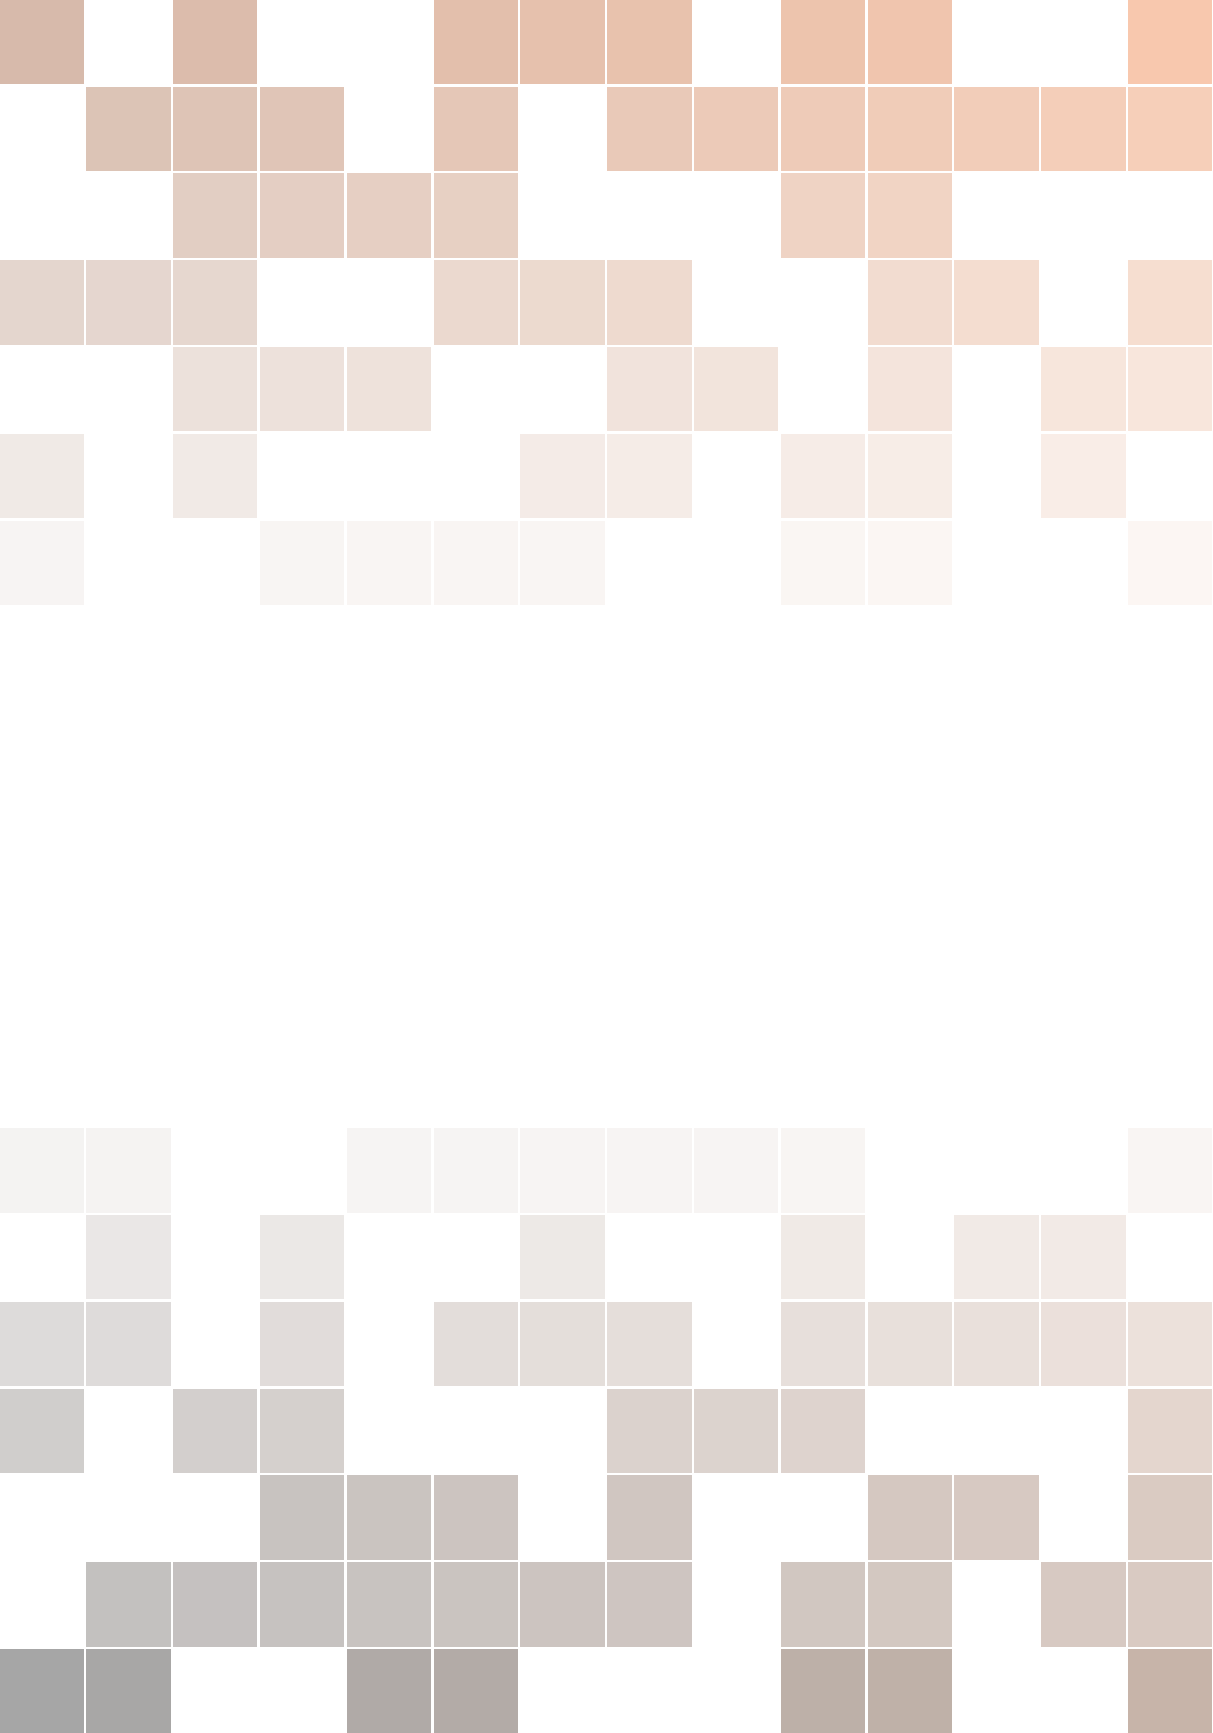
\includegraphics[width=\paperwidth]{background.pdf}};
\draw (current page.center) node [fill=ocre!30!white,fill opacity=0.6,text opacity=1,inner sep=1cm]{\Huge\centering\bfseries\sffamily\parbox[c][][t]{\paperwidth}{\centering Como hacer una maqueta de trenes ...\\[15pt] % Book title
{\Large ... y no perderse en el intento}\\[20pt] % Subtitle
{\huge Daniel Vilas}}}; % Author name
\end{tikzpicture}
\vfill
\endgroup

%----------------------------------------------------------------------------------------
%	COPYRIGHT PAGE
%----------------------------------------------------------------------------------------

\newpage
~\vfill
\thispagestyle{empty}

\noindent Copyright \copyright\ 2021 Daniel Vilas\\ % Copyright notice

\noindent \textsc{Publicado por Self-Pubished}\\ % Publisher

\noindent \textsc{https://mimaquetaarduino.wordpress.com}\\ % URL

\noindent Este trabajo de Daniel Vilas esta licenciado bajo Attribution-NonCommercial 4.0 International. Para ver una copia de la licencia acceda a \url{https://creativecommons.org/licenses/by-nc/4.0/deed.es}. A menos que lo exija la ley aplicable o se acuerde por escrito, el software distribuido bajo la Licencia se distribuye en un \textsc{``tal cual'', sin garantías ni condiciones de ningún tipo}, ya sea expreso o implícito. Consulte la Licencia para conocer el idioma específico que rige los permisos y las limitaciones de la Licencia.\\ % License information, replace this with your own license (if any)

\noindent Editado con \LaTeX{}

\noindent \textit{Primera Impresión, ? 2021} % Printing/edition date

%----------------------------------------------------------------------------------------
%	TABLE OF CONTENTS
%----------------------------------------------------------------------------------------

%\usechapterimagefalse % If you don't want to include a chapter image, use this to toggle images off - it can be enabled later with \usechapterimagetrue

\chapterimage{chapter_head_1.pdf} % Table of contents heading image

\pagestyle{empty} % Disable headers and footers for the following pages
%\renewcommand{\contentsname}{Contenidos}}
\tableofcontents % Print the table of contents itself

\cleardoublepage % Forces the first chapter to start on an odd page so it's on the right side of the book

\pagestyle{fancy} % Enable headers and footers again

%----------------------------------------------------------------------------------------
%	PART
%----------------------------------------------------------------------------------------

\part{Motivación}

\chapterimage{chapter_head_2.pdf} % Chapter heading image

\chapter{Introducción}
% !TeX encoding = UTF-8
% !TeX spellcheck = es_ES
% !TeX root = ../../main.tex

\epigraph{Todo viaje, por largo que sea, empieza por un solo paso}{Lao Tse}

\begin{abstract}
¿Porque este documento? ¿Que es lo que veremos en él? Empezamos un camino, este pdf, post o una maqueta, y por algo hay que empezar. Así que este capitulo trataremos de presentar como orientamos el resto de los capítulos, tanto en forma como en contenidos.
\end{abstract}

\section{Introducción}
La motivación que hay detrás de este trabajo no es otro que ir documentando un viaje con la esperanza de que sirva a otras personas. Este es viaje el del autor mientras crea la maqueta de trenes, a la vez, servirá para ir llenando un sentimiento de necesidad de pulir sus habilidades comunicativas en el formato académico.

En este aspecto se ira escribiendo el texto siguiendo un poco la normativa y estilismos  recomendados para los textos académicos. Potenciando el uso de la pasiva y una estructura que contemple al menos los siguientes apartados, aunque no sean con esos nombres
\begin{itemize}
	\item \textit{Resumen}, una breve explicación del capitulo, lo que se espera de el.
	\item \textit{Introducción}, donde se exponga el problema y situe al lector en contexto.
	\item \textit{Estado del arte}, 
	\item \textit{Experimento} o \textit{Texto principal}
	\item \textit{Resultados}(Opcional) 
	\item \textit{Discusión}
	\item \textit{Conclusiones}
	\item \textit{Próximos pasos}
	\item \textit{Bibliografia} y \textit{Referencias}
\end{itemize}
A lo largo de los   
\cite{acemoglu2000} Es una prueba

\section{Estado del arte}
``No conviene confundir maqueta compacta con óvalo.

Y de ahí que sus diferentes elementos, entre otros:
\begin{itemize}
	\item Tema principal
	\item Forma de la maqueta
	\item Flujo del tráfico
	\item Plano de vías
	\item Orografía
	\item Instalaciones ferroviarias
	\item Circulaciones
\end{itemize}


Es en la meditada ELECCIÓN de todos esos elementos interrelacionados a introducir en la maqueta (y que nunca es sólo EL PLANO DE VÍAS) lo que le dará juego sin fin a la vez que funcionalidad, más allá del grado de destreza y oficio modelísticos. Cuando también estos entran en escena, es cuando se habla de realismo, pero englobando las anteriores, que muchas veces se olvidan.

El foro está llenito de buenas maquetas modulares, módulos, dioramas, maquetas compactas y grandes maquetas.
Y todas las que son admiradas y reciben mayores elogios interrelacionan muy hábilmente los ingredientes anteriormente mencionados.

Y, por la misma razón, la vegetación convincente no se obtiene tanto por su altura a escala, que también, sino quizás más por cómo ese árbol en concreto se relaciona con todo su entorno y su disposición concreta en la maqueta en relación a lo demás.

MODELAR ES ELEGIR CON BISTURÍ: componentes, ángulo de visión, perspectiva y fondo. Y eso es lo que tienen las buenas maquetas, sean grandes, pequeñas, con forma de roscón de reyes o de txapela vasca''` \cite{carrington2021}

\section{Bibliografía}
\printbibliography[heading=subbibliography]


\chapter{Como Jugamos}
% !TeX encoding = UTF-8
% !TeX spellcheck = es_ES
% !TeX root = ../../main.tex


\epigraph{Los hombres no crecen, solo cambian el precio y tamaño de sus juguetes}{Cita anonima en Internet}

\begin{abstract}
Hay varias formas de jugar con una maqueta de tren, en este capitulo se revisaran algunas de las más comunes
\end{abstract}

\section{Introducción}
La mayoría de aficionados, como el autor, empiezan con una caja de iniciación. Montando un óvalo y dando vueltas, lo que sinceramente tras unas cuantas, es un poco más divertido que ver secarse la pintura, aunque no mucho más.

En este momento, el aficionado común, es cuando decide montarse su propia maqueta. Busca el espacio más grande que dispone y en definitiva, siendo su primera maqueta, hace una revisión del óvalo. Más grande, con más vías y desvíos, pero al final se tratará de lo mismo. Dar vueltas.

Lo cierto es que con esta maqueta habrá puesto alguna estación con apartadero, o una playa de vías, o algo con lo que maniobrar. Con esta experiencia acabará haciendo una maqueta nueva que se vaya ajustando a una forma de jugar.

\begin{figure}[h]
	\centering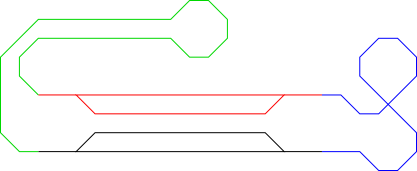
\includegraphics[]{chapters/01_jugar/maqueta.png}
	\caption{Maqueta un poco más compleja (pero un ovalo al fin y acabo)}
	\label{fig:maqueta}
\end{figure}

A este aficionado quizás le guste más simular las operaciones de una línea, o resolver puzzles “time-saver ” o … Al final hay tantas formas de jugar como aficionados. Y la maqueta personal se deberá hacer con forme se piense que se va a jugar con ella.

Este es un proceso que se debe pasar y existen errores que se deben cometer si se quiere disfrutar al máximo. Aunque es posible tomar algún atajo, siempre y cuando al final sepa como va a jugar. Si algún amigo tiene ya una maqueta o siendo socio de un club, tendrá a su disposición unas primeras maquetas con las que aprender cómo jugar.

Otro atajo es leer foros y artículos de revistas. Entorno al 2019/06/03 en forotrenes publicaron unos pdfs hablando sobre una serie de artículos explicando cómo planificaron una maqueta según una explotación realista. Y la conclusión que podemos obtener es la misma. Pensar antes como jugar y el contexto (de la línea imaginada) y luego diseñar la maqueta.

Bueno, teniendo claro que antes de diseñar una maqueta (e incluso antes de buscar el espacio) tenemos que saber como jugar, queremos saber que formas de jugar hay.

\section{Estado del arte}
Unos grupos iniciales de como jugar serán y de los que es fácil encontrar información:

\begin{itemize}
	\item Time-Saver o Puzzles
	\item Cartas o Americano
	\item Explotación o Europeo
	\item Exhibición
\end{itemize}
Así mismo hay otras formas que no se dicen expresamente, pero que se nombran o se intuyen.
\begin{itemize}
	\item Libre
	\item Otras formas Regladas
\end{itemize}
\subsection{Time Saver o Puzzles}
Son maquetas pequeñas y, por norma general, lineales abiertas. Una vía recta recorre toda la longitud y representa la línea principal, de la cual sale una zona de maniobras.
\begin{figure}[h]
	\centering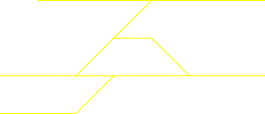
\includegraphics[]{chapters/01_jugar/path4865.png}
	\caption{Ejemplo TimeSaver}
	\label{fig:timesaver} % Unique label used for referencing the figure in-text
	%\addcontentsline{toc}{figure}{Figure \ref{fig:placeholder}} % Uncomment to add the figure to the table of contents
\end{figure}

En la maqueta se colocan una máquina (tractor de maniobras ) y varios vagones, siguiendo una disposición inicial. Además se tiene un plano con la situación final.

El juego se trata que moviendo el tractor, enganchado y desenganchado vagones, cambiando agujas y demás hasta se llegue a la situación final.

La reglas son sencillas, los trenes van por la vía y no se puede usar la mano (salvo desenganches y descarrilamientos). Se puede jugar en solitario, o compitiendo contra otros, en dicho caso, gana quien tarde menos (en tiempo o en pasos).

\subsection{Cartas o Sistema Americano}
Se llama Sistema Americano porque es el preferido en EEUU, se trata de tener todo el material en la maqueta y que todo el mismo se mueva.

A cada vagón se le asigna una tarjeta. En la cual se le asignan 4 destinos y se trata que todos los vagones recorran sus cuatro destinos. El último destino se considera su base y debe ser el punto de inicio.

Para facilitar el juego en cada destino se pone un cajetín con los vagones que tiene. Las cartas son pequeñas y los destinos se escriben de tal forma que girándola carta quede visible en el cajetín el próximo destino del vagón. El operador de dicho destino tiene que hacer una nueva composición y enviar el nuevo tren por una línea que acerque cada vagón a su siguiente destino.

\begin{figure}[h]
	\centering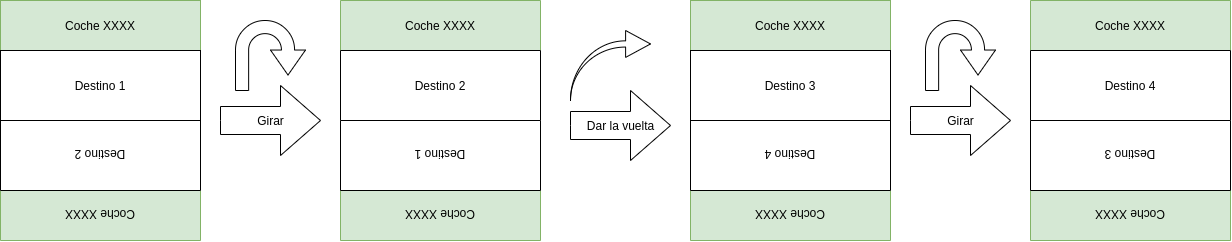
\includegraphics[width=\textwidth]{chapters/01_jugar/HowToPlay-cartas.png}
	\caption{Ejemplo de Carta}
	\label{fig:cartas} % Unique label used for referencing the figure in-text
	%\addcontentsline{toc}{figure}{Figure \ref{fig:placeholder}} % Uncomment to add the figure to the table of contents
\end{figure}

Es necesario tener una maqueta grande, donde incluir múltiples destinos. Y en esos destinos tener una zona para maniobrar donde crear nuevas composiciones. En estados unidos, es mas usual vivir en unifamiliares y tener un sótano más grande donde poner la maqueta.

También se pueden jugar varios encargándose cada uno de una zona (varios destinos)

\subsection{Explotación Real o Sistema Europeo}
Como el anterior, es el preferido en Europa y por eso se llama sistema Europeo. En este caso la maqueta se diseña simulando una línea “real”. El jugador o maquetista sera el dueño de una compañía ficticia. O al menos el responsable de gestionar los trenes para dicha compañía.

Se parte de un contexto o motivo que justifique la misma, sus elementos y su paisaje. Por ejemplo una ciudad pesquera con su estación de termino con comunicaciones a la capital y un pueblo intermedio. En este ejemplo la industria pesquera recibe los pescados del pueblo y los enviá a la capital. La gente de la capital utiliza el pueblo como destino turístico. 

Con estos datos se planificaran las estaciones, dos términos y un apeadero en medio. Así mismo se incluirán las naves de mantenimiento, bases, playas de vías, etc …. Para alargar un poco el juego, se incluirá un ovalo que permita alargar el recorrido. En general es una linea punto a punto, como sucede en la realidad. Si bien se añadido un ovalo en pos de la jugabilidad.

\begin{figure}[h]
	\centering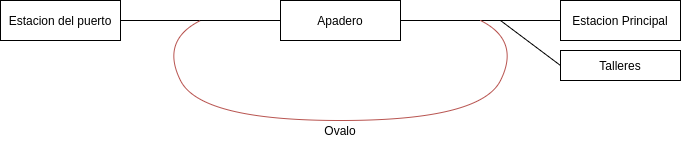
\includegraphics[width=\textwidth]{chapters/01_jugar/HowToPlay-EU.png}
	\caption{Ejemplo de explotación}
	\label{fig:explotacion} % Unique label used for referencing the figure in-text
	%\addcontentsline{toc}{figure}{Figure \ref{fig:placeholder}} % Uncomment to add the figure to the table of contents
\end{figure}

Para jugar con esta maqueta sera conveniente así mismo pensar o definir las reglas de operaciones:

\begin{itemize}
	\item Prioridades de trenes (Alta Velocidad, Pasajeros, Mercancías perecederas, …)
\item Reglas de paso (los trenes mercantes pasan por vías sin anden, la vía no desviada no tiene anden, se reserva para pasos sin parada,…)
\item Reglas de dirección (en doble vía por la derecha, los que van hacia el pueblo pesquero paran en vías pares,…)
\item …
\end{itemize}
También se tendrá que pensar en los trenes regulares (Expresos nocturnos, regionales mercancías, …) como se nombran e identifican. Con esto se podrá crear una tabla de horarios para cada estación.

En ultimo lugar, pero no por ello menos importante, unas reglas para la maqueta o de compresión de la realidad serán necesarias. En el ejemplo, se define que para ir del pueblo a la capital hay que dar 5 vueltas al ovalo, y el apeadero esta en la vuelta 3. Otra regla de compresión, es el reloj acelerado (1 hora en la realidad son 3 en el juego, por ejemplo) o que tal vagón puede cargar X pasajeros o Y toneladas y, por lo tanto, necesita un tiempo definido para carga y descarga.

El objetivo es siempre el mismo: optimizar el uso del material siendo capaces de cumplir la tabla de horarios que se haya definido. Pero se puede complicar todo lo que se quiera (mantenimiento periódico, costes de carburante,…)

Este sistema se prefiere en Europa ya que poca gente tiene un gran espacio donde montar su maqueta y es muy fácil ajustarlo al espacio disponible:

Si tenemos poco espacio podemos diseñar una estación que ocupe lo máximo posible y preocuparlos solamente por gestionar los trenes que entran y salen de ella. Para que el juego sea interesante debe ser una estación principal donde haya que entrar o sacar un tren cada poco y ademas montar y desmontar composiciones, fuera de la estación puede ser una playa de vías con varias composiciones preparadas o montarlas a mano.

Si tenemos mucho espacio podemos hacer una linea completa con varias estaciones, industrias,…

Nos ayudara mucho hacernos un cronograma de donde va estar cada tren en cada momento.

\subsection{Exhibición}

\section{¿Que tenemos ademas?}

\subsection{Libre}
Obviamente lo anterior son las categorías que he ido viendo por internet, luego cada uno se pude organizar como quiera.

En el juego libre movemos nuestros trenes sin una razón ni reglas concretas. Ahora muevo el talgo, luego el mixto, paro este aquí,….

En esta categoría incluyó la exhibición. Y es mover los trenes con el objetivo de que alguien los vea. No solo el propio tren, sino también la maqueta.

Ademas en este apartado podemos hablar de rodaje técnico, o mover las piezas para que la mecánica no se oxide…Paragraph

Esta categoría agrupa todas las formas de jugar que moveremos los trenes sin un sistema de reglas o sin objetivo claro.

\subsection{Otras Formas Regladas}
Aquí agrupo otras formas, no tan extendidas de jugar, pero regladas. Al final cada uno tiene su maqueta y juega como quiere.

Por ejemplo en las exposiciones y encuentro de modelos, se suele hacer una tabla de horarios y unas composiciones y se trata de que cada modulista se encarga de una zona (varios módulos) y se debe cumplir el horario dicho. Amen de otras reglas que dicte el organizador.

Si vamos a un encuentro de módulos como visitantes veremos a un grupo de “amigos” que se mandan trenes de uno a otro, siempre atentos a los trenes y a los controles. Si queremos preguntar algo de la maqueta, nos dirigiremos, o nos responderá alguien que no este a los mandos en ese momento.

Por otra parte si vamos a una exposición, las maquetas las habra hecho una sola persona, o un grupo reducido de personas (en general). Habra un tren dando vueltas, para que se vea como queda. Pero básicamente el tren andará solo, no se parara en las estaciones y el dueño estará vigilando que los visitantes no metan las zarpas (digo las manos) en medio de la maqueta y resolviendo dudas y preguntas de los visitantes.

\section{Resultados o Datos de interés}(Opcional) 
Si es un experimento incluir los datos o resultados obtenidos, sin valorar ni judgar. Es buen lugar para incluir otros detalles encontrados durante la escritura, búsqueda de información,....
\section{Discusión}
Este el punto para valorar los resultados y dar opiniones.
\section{Conclusiones}
Resumir y agrupar los resultados obtenidos
\section{Próximos pasos}
Escribir aquí un breve texto de lo que se hablara en otros capítulos (y que tenga referencia con este), o cosas que se dejan para realizar en un futuro fuera de este PDF.
\section{Bibliografía y Referencias}
\printbibliography[heading=subbibliography]

\part{Ingenieria en la maqueta}
\chapterimage{chapter_head_1.pdf} % Chapter heading image
\chapter{¿Ingenieria?¿en la maqueta?}
\chapter{Requisitos}
% !TeX encoding = UTF-8
% !TeX spellcheck = es_ES
% !TeX root = ../../main.tex

\epigraph{El mundo entero se aparta cuando ve pasar a un hombre que sabe a dónde va}{Antoine de Saint-Exupéry }

\begin{abstract}
    En un proyecto de ingeniería el primer paso es la captura de requisitos.
    Seguramente un perfil mas comercial dirá que el primero es venderlo, pero para venderlo hay que dar un precio
    y para dar ese precio hay que estimar cuanto costara, para ello se necesita saber lo que se quiere,
    ergo los requisitos diría el perfil más técnico, luego seguramente acabarían comentando que si toma o captura
    de requisitos. Según como sea podrán estar así horas y horas para decir lo mismo con distintos términos.
\end{abstract}

\section{Introducción}

En la realidad hay dos momentos donde se recogen los requisitos, en una fase pre-venta se recogen a alto nivel
(por ejemplo que el puente soporte el peso de 10 coches) y una vez contratado el proyecto se realiza otra fase con
más detalle (10 coches coches se convierten en X toneladas suponiendo la media de los que pasan es Y más un margen
de Z\%,…).
Estos dos momentos se suelen llamar toma y captura, pero cada metodología y/o empresa define cual de esos términos
es cada fase, incluso cambiando el nombre.

Es importante realizar esta captura lo antes posible y con el mayor nivel de detalle posible.
Cambiar los requisitos (modificarlos, quitar o añadir alguno) significa revisar todas las decisiones y acciones
realizadas hasta el momento que se puedan ver afectadas por dicha modificación.
Por lo que si se debe realizar los cambios, costara más cuanto más nos acercaremos al final.

Por ejemplo, si inicialmente tenemos un espacio de 3x4 metros y luego cambiamos a 2x3 metros.
No es lo mismo que estemos pensando el diseño de la maqueta, a tener ya las vías pegadas y empezando a hacer
la decoración escénica. Ya que esta es un requisito que afecta a muchas acciones y decisiones.
Por otra parte, otros requisitos pueden cambiarse casi sin afectar.
Imaginémonos que en un principio queremos representar una escena invernal, pero antes de hacer el paisaje se
decide cambiar por una veraniega y el impacto será mínimo puesto que aun no se había empezados.
Ojo, que quizás alguna decisión pudiera ser sido diferente, como podría ser añadir una playa con un puerto
si se hubiera decidido antes.

\section{Estado del arte}
Centrándonos en que esto es para una maqueta y no un proyecto de ingeniería al uso,
no necesitamos toda una disertación de fases, costes, análisis, gestión del cambio, impacto, etc.
Nos tenemos que quedar con la idea de definirlos lo antes posible, puesto que cambiarlo más tarde costara.
Es decir necesitamos tener el listado de requisitos y pensados con cabeza.

Para poder hablar de los requisitos debemos primero, ver lo que son y sus características. Despues en la seccion
de discusion hablaremos en más detalle\footnote{NdA: Siguiendo una estrucutra más academica}.

\subsection{¿Qué son los requisitos?}

En resumen los requisitos son únicamente el listado de cosas que tiene que cumplir la maqueta, o los objetivos
de la misma. En un proyecto de ingenierías se suelen dividir en tipos, como funcionales (Lo que tiene que hacer)
y técnicos (restricciones físicas) para la proyectos informáticos.
Cada ingeniería tiene su propia categoría y aquí estamos en un hobby de maquetas.
Por tanto los organizaremos y clasificaremos por lo que más nos interese.
Si que podría ser interesante tenerlos organizados por intencionalidad (que se quiere lograr),
escénico (tener tal y tal cosa) y físicos (donde debe caber u otras limitaciones realacioandos con espacio).

Es muy importante tener en cuenta que los requisitos son lo que luego que dictaminarán si una maqueta es un
éxito y por tanto buena. Dicho de otra forma, será una buena maqueta si cumple los requisitos u objetivos
planteados. Así que dichos requisitos deben estar escritos en algún sitio.

Los requisitos siempre responden a preguntas del tipo ¿Qué quiero…? ¿Dónde quiero…?
O ¿Qué debe …? O ¿Dónde debe…?

Algunos requisitos estarán muy relacionados entre si, quizás siendo aclaraciones o detalles de uno.
Por lo que podremos considerarlos como Sub-requisitos.

\subsection{Objetivos y Prioridades}

Los objetivos son los requisitos que nos parecen más importantes y son lo que consideramos básicos que
la maqueta debe cumplir. Son particulares de cada maquetista y ninguno es trivial. Básicamente responden
¿Qué quiero conseguir con mi maqueta? Aunque al final serán los que se consideren más importantes.

Como se puede intuir, no todos los requisitos será igual de importantes, y los menos importantes podremos
no cumplirlos o modificarlos para que se ajusten a lo que tenemos creado. Pero los más importantes deberemos
mantenerlos lo más fijos posibles.

\subsection{Detalle de los requisitos}

Los requisitos deberían ser breves, concisos, concretos y claros. Pero a su vez deben tener el mayor detalle
posible para que sea lo más fácil posible tomar las decisiones futuras. Por ejemplo veamos posibles requisitos,
que son el mismo, pero con diferente nivel de detalle.

\begin{enumerate}
    \item Quiero un parque de atracciones.
    \item Quiero un parque de atracciones inspirado en el de mi ciudad
    \item Quiero un parque de atracciones con una noria y un lago.
    \item Quiero un parque de atracciones con una noria modelo tal y un lago que tenga 3 barcas modelo tal.
    \item Quiero un parque de atracciones inspirado en el de mi cuidad, con al menos las atracciones … y siguiendo el mapa …
\end{enumerate}

Como podemos ver el número 1 es el más genérico y abstracto, pero también nos permite más flexibilidad en
decisiones futuras. Por otra parte el 4 y el 5 son los más concretos y con más detalle, son más rígidos
pero por otra parte nos fija cosas que luego nos evitamos pensar.

En el caso del 5, incluso convendría, partir el listado de atracciones en Sub-requisitos para que no quede muy
largo el mismo, pero considerarlos todos como uno, si va a ser un objetivo de la maqueta.

\subsection{Cuando tener los requisitos}

Los requisitos deben estar lo antes posible y siempre antes de que comiencen a necesitarse.
Los requisitos serán la plantilla para la toma de decisiones como la elección entre alternativas.
Por lo tanto no es necesario tener todos al principio, pero si los objetivos.

Volviendo al ejemplo anterior, suponiendo que hacemos una maqueta por módulos y vamos a tratar el modulo
donde pondremos el parque de atracciones. Realmente hasta este momento no hemos necesitado el requisito hasta
este momento, por lo tanto podremos no tenerlo o modificarlo ”sin coste” hasta ahora.
Pero si lo modificamos después de hacer el modulo, puede que tengamos que rehacerlo.

Es decir necesitaremos tener el requisito lo más detallado junto antes de usarlo, pero en el listado de
requisitos debería estar, aunque sea con baja definición, desde el momento se nos pase por la cabeza.

En el ejemplo del parque de atracciones, tendríamos el 1 al principio, más adelante cuando se planifiquen
los módulos, algo un poco más detallado como el 2 o 3, para dar una idea más clara.
Pero el momento de diseñar el modulo concreto el 4 o 5.
\subsection{Requisitos de espacio}

\section{Ejemplo Practico}
\section{Texto principal}

\section{Resultados}
%\subsection{Los requisitos de una maqueta}

La maqueta que queremos desarrollar será sobre una empresa ficticia DanielBahn y el resultado final será
el resultado de varios años de trabajo, en este momento y estos artículos se describe el proceso para un
maqueta más pequeña DanielTeppichBahn\footnote{TeppichBahn es como llaman en Alemania a las maquetas de
    tren que se montan sobre el suelo para jugar y se desmontan cuando ya se ha acabado el juego.}.
Aunque, teniendo que esta maqueta será para probar técnicas/tecnologías para la versión final.
Se tendrán en cuenta en los requisitos.

El proceso para tener los requisitos es iterativo, es decir se van escribiendo en iteraciones,
intentando ir ampliando poco a poco para cada maqueta.

Para DanielBahn tenemos los objetivos  siguientes:
\begin{itemize}
    \item Representar tres escenas inspiradas en sitios reales, por importancia sentimental
          \begin{itemize}
              \item La estación del puerto de La Coruña hasta la playa de lazareto
              \item La estación del Santo Sepulcro de Zaragoza
              \item Una estación de montaña como la de Canfranc
          \end{itemize}
    \item Desarrollar módulos electrónicos en LCC para desvíos, y paneles de control.
    \item DCC para las vias y para los mandos, cualquiera con soporte para JMRI
    \item Tener un una vía continua para realizar fotos, sin preocupaciones de tener que evitar choques contra fin de vía
    \item Tener una zona de puzzle de clasificación
    \item Ser más o menos realista en trazado y operación.
\end{itemize}


Como se puede ver son lo suficientemente concretos para poder ir diseñando y pensando alternativas,
pero tan genéricos que dan lugar multitud de opciones. Así mismo es tan a largo plazo, que es más una lista de
deseos que un listado de requisitos al uso. Tampoco hay restricciones de espacio, a la espera de realizar diseños
y buscar alternativas.

DanielTeppichBahn, por su parte será una maqueta para poner en el suelo, y de aprendizaje por los que sus
objetivos son:
\begin{itemize}
    \item Tener una maqueta pequeña para:

          \begin{itemize}
              \item Rodar los trenes
              \item Aprender técnicas
              \item Probar nuevas ideas
          \end{itemize}
    \item Debe caber “escondida” detrás de un mueble:
    \item Debe ser fácil de montar
    \item Con Electrónica para controlar desvíos, y luces hecha por mi.
    \item Debe tener los problemas típicos(Si es posible):

          \begin{itemize}
              \item Playa de vías
              \item Vías de escape
              \item Cruces
              \item Bucles
          \end{itemize}
    \item DCC para las vías y los desvíos
    \item Loconet para los mandos, módulos propios para JMRI
    \item Paneles y módulos propios en Loconet (para ahorrar cables)
    \item Basada en montaje de caja inicial
\end{itemize}

Como se puede apreciar, en esta maqueta ya aparece un requisito donde debe estar guardada, porque es el compromiso
que hemos podido llegar, para tener una maqueta. Y son más concretos, con lo que nos permite ir desarrollando
esta maqueta.

Seguramente, iremos desarrollando maquetas según el tiempo y el espacio disponible vayan variando.
\section{Discusión}
\subsection{Requisitos de espacio}

Las limitaciones de espacio, y por ende sus requisitos, se suelen tener en cuenta antes si quiera de empezar
a pensar en la maqueta. Esto es un reflejo de las situación de cuando podemos hacer la maqueta.
Normalmente cuando tenemos ya la vida resuelta y el espacio ocupado ya en la casa por estanterías, muebles
y demás.

Esto nos obliga a hacer compromisos, con otras personas, el espacio y lo que queríamos hacer, por lo que
muchas veces acabamos con una maqueta que no nos satisface del todo. Desde este apartado, abogamos por
retrasar estos requisitos lo máximo posible hasta una fase de análisis y diseño con los requisitos que se
realmente se quiere.

Para poder retrasar estos requisitos necesitamos una fase de análisis y diseño, donde veremos el espacio
que requiriéramos para el resto de requisitos y nos obligará a pensar alternativas de espacio
(alquilar un local, usar la casa del pueblo, mudarse, …), pensar en diseños para varias habitaciones, o
un cambio de diseño (pasar a escenas en varios niveles, segmentada, de maleta,…).

También nos permite probar varios diseños, sobre el papel o sobre pruebas, donde llegaremos a compromisos,
con la seguridad que hemos intentando todo lo posible por tener todo aquello que queríamos necesariamente.
Y que ademas ha sido imposible tener más.

Esto no quiere decir que tener requisitos de espacio al principio sea malo. Los tendremos si es algo ”fijo”
puesto que se ha acordado previamente con otras personas del hogar, o porque es la única posibilidad real.
Pero recordemos que luego un cambio de esto, tiene grandes implicaciones, por lo que cuanto más tarde 
lo tengamos mejor. Aunque implicara pensar más alternativas y por lo tanto más trabajo intelectual.

\section{Conclusiones}
Como hemos comentado, lo importante de los requisitos es tener un documento o listado de lo que se quiere
tener. Este listado debe ser lo mas detallado posible, pero cuando se necesite. Al principio lo tendremos 
con poco detalle y lo iremos detallando a necesidad. Nos preocuparemos más de lo que queremos y las
limitaciones intentaremos retrasarlas para buscar alternativas.

También hemos presentado los objetivos de la maqueta final, a largo plazo (DanielBahn) y otra mas cercana
en el tiempo para ir aprendiendo y tener un sitio donde rodar (DanielTeppichBahn)

Como conclusión, tengamos sentido común, y hagamos una lista de lo que realmente queramos y luego
estudiemos opciones para ver como podemos llegar a ellas. No tengamos miedo a pensar a largo plazo y
hacer maquetas intermedias para aprender, o probar cosas. 
\section{Próximos pasos}

\section{Bibliografía}
\printbibliography[heading=subbibliography]


\part{Normativa}
\chapterimage{chapter_head_2.pdf} % Chapter heading image

\chapter{Introducción a las normativas}
% !TeX encoding = UTF-8
% !TeX spellcheck = es_ES
% !TeX root = ../../main.tex

\epigraph{Todo viaje, por largo que sea, empieza por un solo paso}{Lao Tse}

\begin{abstract}
¿Porque este documento? ¿Que es lo que veremos en él? Empezamos un camino, este pdf, post o una maqueta, y por algo hay que empezar. Así que este capitulo trataremos de presentar como orientamos el resto de los capítulos, tanto en forma como en contenidos.
\end{abstract}

\section{Introducción}
La motivación que hay detrás de este trabajo no es otro que ir documentando un viaje con la esperanza de que sirva a otras personas. Este es viaje el del autor mientras crea la maqueta de trenes, a la vez, servirá para ir llenando un sentimiento de necesidad de pulir sus habilidades comunicativas en el formato académico.

En este aspecto se ira escribiendo el texto siguiendo un poco la normativa y estilismos  recomendados para los textos académicos. Potenciando el uso de la pasiva y una estructura que contemple al menos los siguientes apartados, aunque no sean con esos nombres
\begin{itemize}
	\item \textit{Resumen}, una breve explicación del capitulo, lo que se espera de el.
	\item \textit{Introducción}, donde se exponga el problema y situe al lector en contexto.
	\item \textit{Estado del arte}, 
	\item \textit{Experimento} o \textit{Texto principal}
	\item \textit{Resultados}(Opcional) 
	\item \textit{Discusión}
	\item \textit{Conclusiones}
	\item \textit{Próximos pasos}
	\item \textit{Bibliografia} y \textit{Referencias}
\end{itemize}
A lo largo de los   
\cite{acemoglu2000} Es una prueba

\section{Estado del arte}
``No conviene confundir maqueta compacta con óvalo.

Y de ahí que sus diferentes elementos, entre otros:
\begin{itemize}
	\item Tema principal
	\item Forma de la maqueta
	\item Flujo del tráfico
	\item Plano de vías
	\item Orografía
	\item Instalaciones ferroviarias
	\item Circulaciones
\end{itemize}


Es en la meditada ELECCIÓN de todos esos elementos interrelacionados a introducir en la maqueta (y que nunca es sólo EL PLANO DE VÍAS) lo que le dará juego sin fin a la vez que funcionalidad, más allá del grado de destreza y oficio modelísticos. Cuando también estos entran en escena, es cuando se habla de realismo, pero englobando las anteriores, que muchas veces se olvidan.

El foro está llenito de buenas maquetas modulares, módulos, dioramas, maquetas compactas y grandes maquetas.
Y todas las que son admiradas y reciben mayores elogios interrelacionan muy hábilmente los ingredientes anteriormente mencionados.

Y, por la misma razón, la vegetación convincente no se obtiene tanto por su altura a escala, que también, sino quizás más por cómo ese árbol en concreto se relaciona con todo su entorno y su disposición concreta en la maqueta en relación a lo demás.

MODELAR ES ELEGIR CON BISTURÍ: componentes, ángulo de visión, perspectiva y fondo. Y eso es lo que tienen las buenas maquetas, sean grandes, pequeñas, con forma de roscón de reyes o de txapela vasca''` \cite{carrington2021}

\section{Bibliografía}
\printbibliography[heading=subbibliography]

\chapter{Normativa General}

\part{Original}

%%% EXAMPLES
% !TeX root = main.tex
% !TeX encoding = UTF-8
% !TeX spellcheck = es_ES

\part{Examples}
%----------------------------------------------------------------------------------------
%	CHAPTER 1
%----------------------------------------------------------------------------------------

\chapterimage{chapter_head_2.pdf} % Chapter heading image

\chapter{Text Chapter}

\section{Paragraphs of Text}\index{Paragraphs of Text}

\lipsum[1-7] % Dummy text

%------------------------------------------------

\section{Citation}\index{Citation}

This statement requires citation \cite{article_key}; this one is more specific \cite[162]{book_key}.

%------------------------------------------------

\section{Lists}\index{Lists}

Lists are useful to present information in a concise and/or ordered way\footnote{Footnote example...}.

\subsection{Numbered List}\index{Lists!Numbered List}

\begin{enumerate}
	\item The first item
	\item The second item
	\item The third item
\end{enumerate}

\subsection{Bullet Points}\index{Lists!Bullet Points}

\begin{itemize}
	\item The first item
	\item The second item
	\item The third item
\end{itemize}

\subsection{Descriptions and Definitions}\index{Lists!Descriptions and Definitions}

\begin{description}
	\item[Name] Description
	\item[Word] Definition
	\item[Comment] Elaboration
\end{description}

%----------------------------------------------------------------------------------------
%	CHAPTER 2
%----------------------------------------------------------------------------------------

\chapter{In-text Elements}

\section{Theorems}\index{Theorems}

This is an example of theorems.

\subsection{Several equations}\index{Theorems!Several Equations}
This is a theorem consisting of several equations.

\begin{theorem}[Name of the theorem]
	In $E=\mathbb{R}^n$ all norms are equivalent. It has the properties:
	\begin{align}
		& \big| ||\mathbf{x}|| - ||\mathbf{y}|| \big|\leq || \mathbf{x}- \mathbf{y}||\\
		&  ||\sum_{i=1}^n\mathbf{x}_i||\leq \sum_{i=1}^n||\mathbf{x}_i||\quad\text{where $n$ is a finite integer}
	\end{align}
\end{theorem}

\subsection{Single Line}\index{Theorems!Single Line}
This is a theorem consisting of just one line.

\begin{theorem}
	A set $\mathcal{D}(G)$ in dense in $L^2(G)$, $|\cdot|_0$. 
\end{theorem}

%------------------------------------------------

\section{Definitions}\index{Definitions}

This is an example of a definition. A definition could be mathematical or it could define a concept.

\begin{definition}[Definition name]
	Given a vector space $E$, a norm on $E$ is an application, denoted $||\cdot||$, $E$ in $\mathbb{R}^+=[0,+\infty[$ such that:
	\begin{align}
		& ||\mathbf{x}||=0\ \Rightarrow\ \mathbf{x}=\mathbf{0}\\
		& ||\lambda \mathbf{x}||=|\lambda|\cdot ||\mathbf{x}||\\
		& ||\mathbf{x}+\mathbf{y}||\leq ||\mathbf{x}||+||\mathbf{y}||
	\end{align}
\end{definition}

%------------------------------------------------

\section{Notations}\index{Notations}

\begin{notation}
	Given an open subset $G$ of $\mathbb{R}^n$, the set of functions $\varphi$ are:
	\begin{enumerate}
		\item Bounded support $G$;
		\item Infinitely differentiable;
	\end{enumerate}
	a vector space is denoted by $\mathcal{D}(G)$. 
\end{notation}

%------------------------------------------------

\section{Remarks}\index{Remarks}

This is an example of a remark.

\begin{remark}
	The concepts presented here are now in conventional employment in mathematics. Vector spaces are taken over the field $\mathbb{K}=\mathbb{R}$, however, established properties are easily extended to $\mathbb{K}=\mathbb{C}$.
\end{remark}

%------------------------------------------------

\section{Corollaries}\index{Corollaries}

This is an example of a corollary.

\begin{corollary}[Corollary name]
	The concepts presented here are now in conventional employment in mathematics. Vector spaces are taken over the field $\mathbb{K}=\mathbb{R}$, however, established properties are easily extended to $\mathbb{K}=\mathbb{C}$.
\end{corollary}

%------------------------------------------------

\section{Propositions}\index{Propositions}

This is an example of propositions.

\subsection{Several equations}\index{Propositions!Several Equations}

\begin{proposition}[Proposition name]
	It has the properties:
	\begin{align}
		& \big| ||\mathbf{x}|| - ||\mathbf{y}|| \big|\leq || \mathbf{x}- \mathbf{y}||\\
		&  ||\sum_{i=1}^n\mathbf{x}_i||\leq \sum_{i=1}^n||\mathbf{x}_i||\quad\text{where $n$ is a finite integer}
	\end{align}
\end{proposition}

\subsection{Single Line}\index{Propositions!Single Line}

\begin{proposition} 
	Let $f,g\in L^2(G)$; if $\forall \varphi\in\mathcal{D}(G)$, $(f,\varphi)_0=(g,\varphi)_0$ then $f = g$. 
\end{proposition}

%------------------------------------------------

\section{Examples}\index{Examples}

This is an example of examples.

\subsection{Equation and Text}\index{Examples!Equation and Text}

\begin{example}
	Let $G=\{x\in\mathbb{R}^2:|x|<3\}$ and denoted by: $x^0=(1,1)$; consider the function:
	\begin{equation}
		f(x)=\left\{\begin{aligned} & \mathrm{e}^{|x|} & & \text{si $|x-x^0|\leq 1/2$}\\
			& 0 & & \text{si $|x-x^0|> 1/2$}\end{aligned}\right.
	\end{equation}
	The function $f$ has bounded support, we can take $A=\{x\in\mathbb{R}^2:|x-x^0|\leq 1/2+\epsilon\}$ for all $\epsilon\in\intoo{0}{5/2-\sqrt{2}}$.
\end{example}

\subsection{Paragraph of Text}\index{Examples!Paragraph of Text}

\begin{example}[Example name]
	\lipsum[2]
\end{example}

%------------------------------------------------

\section{Exercises}\index{Exercises}

This is an example of an exercise.

\begin{exercise}
	This is a good place to ask a question to test learning progress or further cement ideas into students' minds.
\end{exercise}

%------------------------------------------------

\section{Problems}\index{Problems}

\begin{problem}
	What is the average airspeed velocity of an unladen swallow?
\end{problem}

%------------------------------------------------

\section{Vocabulary}\index{Vocabulary}

Define a word to improve a students' vocabulary.

\begin{vocabulary}[Word]
	Definition of word.
\end{vocabulary}

%----------------------------------------------------------------------------------------
%	PART
%----------------------------------------------------------------------------------------

\part{Part Two}

%----------------------------------------------------------------------------------------
%	CHAPTER 3
%----------------------------------------------------------------------------------------

\chapterimage{chapter_head_1.pdf} % Chapter heading image

\chapter{Presenting Information}

\section{Table}\index{Table}

\begin{table}[h]
	\centering
	\begin{tabular}{l l l}
		\toprule
		\textbf{Treatments} & \textbf{Response 1} & \textbf{Response 2}\\
		\midrule
		Treatment 1 & 0.0003262 & 0.562 \\
		Treatment 2 & 0.0015681 & 0.910 \\
		Treatment 3 & 0.0009271 & 0.296 \\
		\bottomrule
	\end{tabular}
	\caption{Table caption}
	\label{tab:example} % Unique label used for referencing the table in-text
	%\addcontentsline{toc}{table}{Table \ref{tab:example}} % Uncomment to add the table to the table of contents
\end{table}

Referencing Table \ref{tab:example} in-text automatically.

%------------------------------------------------

\section{Figure}\index{Figure}

\begin{figure}[h]
	\centering
\includegraphics[scale=0.5]{placeholder.jpg}
	\caption{Figure caption}
	\label{fig:placeholder} % Unique label used for referencing the figure in-text
	%\addcontentsline{toc}{figure}{Figure \ref{fig:placeholder}} % Uncomment to add the figure to the table of contents
\end{figure}

Referencing Figure \ref{fig:placeholder} in-text automatically.

\chapter{Base}
% !TeX encoding = UTF-8
% !TeX spellcheck = es_ES
% !TeX root = ../../main.tex


\epigraph{Los hombres no crecen, solo cambian el precio y tamaño de sus juguetes}{Cita anonima en Internet}

\begin{abstract}
Hay varias formas de jugar con una maqueta de tren, en este capitulo revisaremos algunas de las más comunes
\end{abstract}

\section{Introducción}
Incluir aquí una introducción al capitulo, estableciendo un contexto para centrar al lector
\cite{ackerberg2006} Es una prueba solo para jugar

\section{Estado del arte}
Explicar como esta actualmente el hobby o las diferentes publicaciones respecto al tema
\section{Experimento o Texto principal}
Describir de la manera más aseptica posible lo que se quiere avanzar
\section{Resultados o Datos de interés}(Opcional) 
Si es un experimento incluir los datos o resultados obtenidos, sin valorar ni judgar. Es buen lugar para incluir otros detalles encontrados durante la escritura, búsqueda de información,....
\section{Discusión}
Este el punto para valorar los resultados y dar opiniones.
\section{Conclusiones}
Resumir y agrupar los resultados obtenidos
\section{Próximos pasos}
Escribir aquí un breve texto de lo que se hablara en otros capítulos (y que tenga referencia con este), o cosas que se dejan para realizar en un futuro fuera de este PDF.
\section{Bibliografía y Referencias}
\printbibliography[heading=subbibliography]
%----------------------------------------------------------------------------------------
%	BIBLIOGRAPHY
%----------------------------------------------------------------------------------------

\chapter*{Bibliography}
\nocite{*}
\addcontentsline{toc}{chapter}{\textcolor{ocre}{Bibliography}} % Add a Bibliography heading to the table of contents

%------------------------------------------------

\section*{Articles}
\addcontentsline{toc}{section}{Articles}
\printbibliography[segment=*,heading=bibempty,type=article]

%------------------------------------------------

\section*{Books}
\addcontentsline{toc}{section}{Books}
\printbibliography[heading=bibempty,type=book]

\section*{Paginas Web}
\addcontentsline{toc}{section}{Paginas Web}
\printbibliography[heading=bibempty,type=online]

%----------------------------------------------------------------------------------------
%	INDEX
%----------------------------------------------------------------------------------------

\cleardoublepage % Make sure the index starts on an odd (right side) page
\phantomsection
\setlength{\columnsep}{0.75cm} % Space between the 2 columns of the index
\addcontentsline{toc}{chapter}{\textcolor{ocre}{Index}} % Add an Index heading to the table of contents
\printindex % Output the index

%----------------------------------------------------------------------------------------

\end{document}
